\documentclass[tikz,border=3pt]{standalone}
\usepackage{amsmath}
\usepackage[dvipsnames]{xcolor}
\usetikzlibrary{arrows.meta,backgrounds,calc,fit,positioning}

\begin{document}
\newcommand{\boxtitle}[1]{{\sffamily\bfseries\fontsize{6.8}{7.2}\selectfont #1}}
\newcommand{\resblock}{\textcolor{teal!70!black}{\mathbf{R}}}
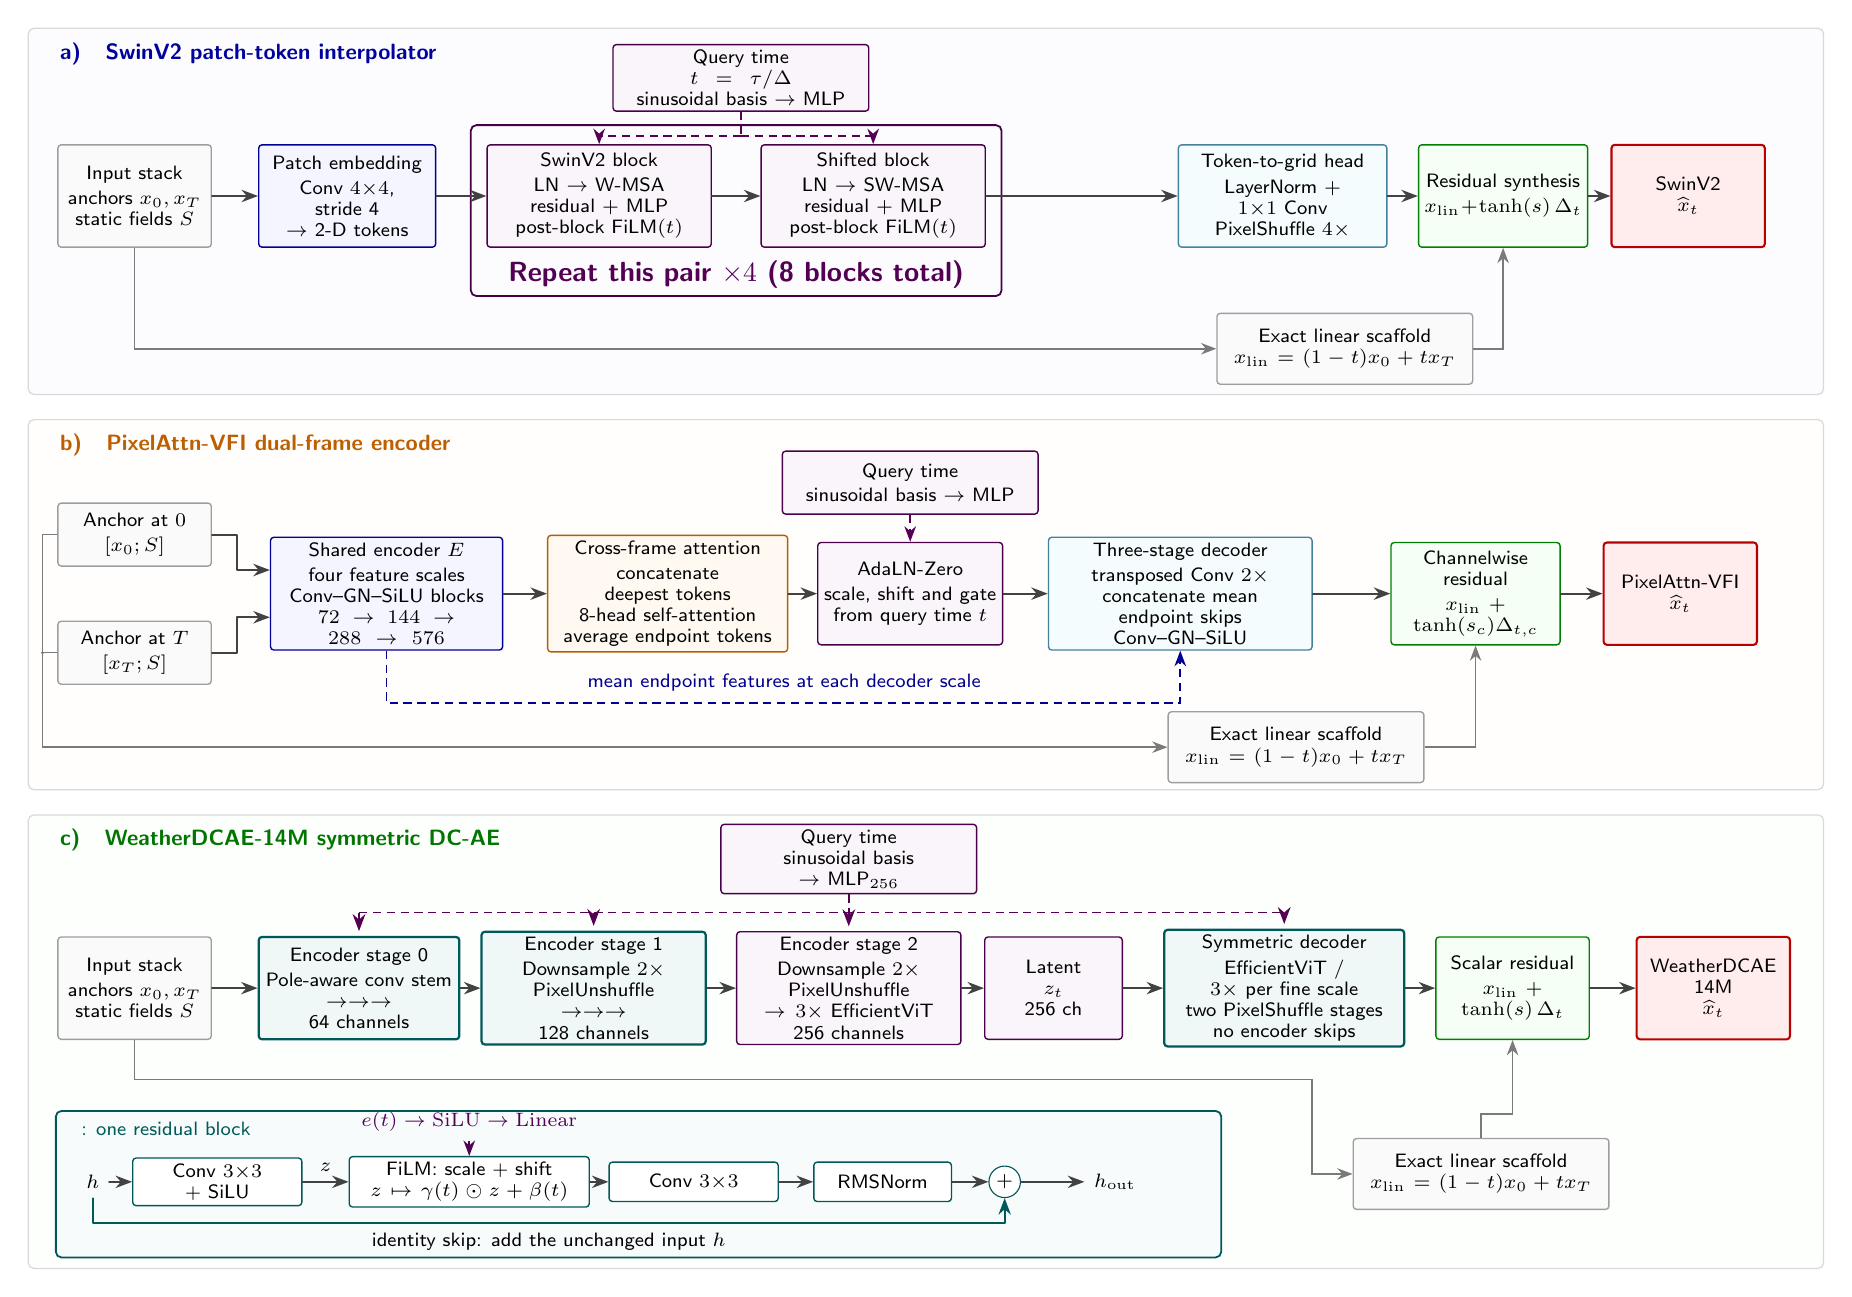
\begin{tikzpicture}[
  x=1cm,
  y=1cm,
  >={Stealth[length=1.7mm,width=1.1mm]},
  font=\sffamily\fontsize{7.0}{7.6}\selectfont,
  box/.style={
    rectangle,
    rounded corners=1.2pt,
    draw=black!38,
    fill=white,
    align=center,
    inner xsep=2.1pt,
    inner ysep=2.0pt,
    minimum height=13mm,
    line width=0.50pt
  },
  input/.style={box,fill=black!2,text width=18mm},
  embed/.style={box,fill=blue!4,draw=blue!58!black,text width=21mm},
  encoder/.style={box,fill=blue!4,draw=blue!58!black,text width=23mm},
  token/.style={box,fill=violet!4,draw=violet!58!black,text width=25mm},
  attention/.style={box,fill=orange!5,draw=orange!72!black,text width=26mm},
  decoder/.style={box,fill=cyan!4,draw=cyan!58!black,text width=25mm},
  residual/.style={box,fill=green!4,draw=green!50!black,text width=21mm},
  scaffold/.style={box,fill=black!2,text width=23mm,minimum height=9mm},
  output/.style={box,fill=red!7,draw=red!72!black,text width=18mm,line width=0.75pt},
  time/.style={box,fill=violet!4,draw=violet!58!black,text width=24mm,minimum height=8mm},
  note/.style={box,fill=white,text width=32mm,minimum height=8mm,font=\sffamily\fontsize{6.8}{7.2}\selectfont},
  rstage/.style={fill=teal!6,draw=teal!70!black,line width=0.8pt},
  rop/.style={box,minimum height=5mm,text width=20mm,fill=white,draw=teal!70!black},
  flow/.style={-Stealth,draw=black!74,line width=0.66pt,line cap=round,line join=round},
  condition/.style={-Stealth,draw=violet!67!black,densely dashed,line width=0.58pt},
  skip/.style={-Stealth,draw=blue!57!black,densely dashed,line width=0.58pt},
  bypass/.style={-Stealth,draw=black!52,line width=0.56pt},
  title/.style={anchor=west,font=\sffamily\bfseries\fontsize{8.2}{8.7}\selectfont},
  boxtitle/.style={font=\sffamily\bfseries\fontsize{6.8}{7.2}\selectfont}
]

% Panel backgrounds.
\begin{scope}[on background layer]
  \fill[blue!1.2,rounded corners=2pt] (0,10.20) rectangle (22.80,14.85);
  \draw[black!15,rounded corners=2pt,line width=0.45pt] (0,10.20) rectangle (22.80,14.85);
  \fill[orange!0.9,rounded corners=2pt] (0,5.18) rectangle (22.80,9.88);
  \draw[black!15,rounded corners=2pt,line width=0.45pt] (0,5.18) rectangle (22.80,9.88);
  \fill[green!0.9,rounded corners=2pt] (0,-0.90) rectangle (22.80,4.86);
  \draw[black!15,rounded corners=2pt,line width=0.45pt] (0,-0.90) rectangle (22.80,4.86);
  \filldraw[fill=teal!3,draw=teal!70!black,rounded corners=2pt,line width=0.65pt]
    (0.35,-0.76) rectangle (15.15,1.10);
\end{scope}

% a) SwinV2.
\node[title,text=blue!62!black] at (0.28,14.53)
  {\textbf{a)}\quad SwinV2 patch-token interpolator};

\node[input] (swin-in) at (1.35,12.72)
  {\boxtitle{Input stack}\\[1.5pt]
   anchors $x_0,x_T$\\static fields $S$};
\node[embed] (swin-patch) at (4.05,12.72)
  {\boxtitle{Patch embedding}\\[1.5pt]
   Conv $4{\times}4$, stride 4\\$\rightarrow$ 2-D tokens};
\node[token,text width=27mm] (swin-w) at (7.25,12.72)
  {\boxtitle{SwinV2 block}\\[1.5pt]
   LN $\rightarrow$ W-MSA\\residual $+$ MLP\\post-block FiLM$(t)$};
\node[token,text width=27mm] (swin-sw) at (10.73,12.72)
  {\boxtitle{Shifted block}\\[1.5pt]
   LN $\rightarrow$ SW-MSA\\residual $+$ MLP\\post-block FiLM$(t)$};
\draw[draw=violet!55!black,rounded corners=2pt,line width=0.65pt]
  (5.62,11.45) rectangle (12.36,13.62);
\node[font=\sffamily\bfseries,text=violet!65!black] at (8.99,11.72)
  {Repeat this pair $\times4$ (8 blocks total)};
\node[decoder,text width=25mm] (swin-up) at (15.93,12.72)
  {\boxtitle{Token-to-grid head}\\[1.5pt]
   LayerNorm $+$ $1{\times}1$ Conv\\PixelShuffle $4{\times}$};
\node[residual,text width=20mm] (swin-mix) at (18.73,12.72)
  {\boxtitle{Residual synthesis}\\[1.5pt]
   $x_{\rm lin}+\tanh(s)\,\Delta_t$};
\node[output] (swin-out) at (21.08,12.72)
  {\boxtitle{SwinV2}\\$\widehat{x}_t$};
\node[time,text width=31mm] (swin-time) at (9.05,14.22)
  {\boxtitle{Query time}\\$t=\tau/\Delta$\\sinusoidal basis $\rightarrow$ MLP};
\node[scaffold,text width=31mm] (swin-lin) at (16.72,10.78)
  {\boxtitle{Exact linear scaffold}\quad
   $x_{\rm lin}=(1-t)x_0+t x_T$};

\draw[flow] (swin-in.east) -- (swin-patch.west);
\draw[flow] (swin-patch.east) -- (swin-w.west);
\draw[flow] (swin-w.east) -- (swin-sw.west);
\draw[flow] (swin-sw.east) -- (swin-up.west);
\draw[flow] (swin-up.east) -- (swin-mix.west);
\draw[flow] (swin-mix.east) -- (swin-out.west);
\draw[condition,-] (swin-time.south) -- (9.05,13.48);
\draw[condition] (9.05,13.48) -| (swin-w.north);
\draw[condition] (9.05,13.48) -| (swin-sw.north);
\draw[bypass] (swin-in.south) |- (swin-lin.west);
\draw[bypass] (swin-lin.east) -| (swin-mix.south);

% b) PixelAttn-VFI.
\node[title,text=orange!74!black] at (0.28,9.56)
  {\textbf{b)}\quad PixelAttn-VFI dual-frame encoder};

\node[input,minimum height=8mm] (pix-in0) at (1.35,8.42)
  {\boxtitle{Anchor at $0$}\\[1.5pt]$[x_0;S]$};
\node[input,minimum height=8mm] (pix-inT) at (1.35,6.92)
  {\boxtitle{Anchor at $T$}\\[1.5pt]$[x_T;S]$};
\node[encoder,text width=28mm] (pix-enc) at (4.55,7.67)
  {\boxtitle{Shared encoder $E$}\\[1.5pt]
   four feature scales\\Conv--GN--SiLU blocks\\$72\rightarrow144\rightarrow288\rightarrow576$};
\node[attention,text width=29mm] (pix-attn) at (8.12,7.67)
  {\boxtitle{Cross-frame attention}\\[1.5pt]
   concatenate deepest tokens\\8-head self-attention\\average endpoint tokens};
\node[token,text width=22mm] (pix-time) at (11.20,7.67)
  {\boxtitle{AdaLN-Zero}\\[1.5pt]
   scale, shift and gate\\from query time $t$};
\node[decoder,text width=32mm] (pix-dec) at (14.63,7.67)
  {\boxtitle{Three-stage decoder}\\[1.5pt]
   transposed Conv $2{\times}$\\concatenate mean endpoint skips\\Conv--GN--SiLU};
\node[residual,text width=20mm] (pix-mix) at (18.38,7.67)
  {\boxtitle{Channelwise residual}\\[1.5pt]
   $x_{\rm lin}+\tanh(s_c)\Delta_{t,c}$};
\node[output] (pix-out) at (20.98,7.67)
  {\boxtitle{PixelAttn-VFI}\\$\widehat{x}_t$};
\node[time,text width=31mm] (pix-query) at (11.20,9.08)
  {\boxtitle{Query time}\\[1pt]sinusoidal basis $\rightarrow$ MLP};
\node[scaffold,text width=31mm] (pix-lin) at (16.10,5.72)
  {\boxtitle{Exact linear scaffold}\quad
   $x_{\rm lin}=(1-t)x_0+t x_T$};

\draw[flow] (pix-in0.east) -- (2.65,8.42) |- ($(pix-enc.west)+(0,0.30)$);
\draw[flow] (pix-inT.east) -- (2.65,6.92) |- ($(pix-enc.west)-(0,0.30)$);
\draw[flow] (pix-enc.east) -- (pix-attn.west);
\draw[flow] (pix-attn.east) -- (pix-time.west);
\draw[flow] (pix-time.east) -- (pix-dec.west);
\draw[flow] (pix-dec.east) -- (pix-mix.west);
\draw[flow] (pix-mix.east) -- (pix-out.west);
\draw[condition] (pix-query.south) -- (pix-time.north);
\draw[skip] (pix-enc.south) -- (4.55,6.28) -- (14.63,6.28) -- (pix-dec.south);
\node[anchor=south,font=\sffamily\fontsize{6.8}{7.2}\selectfont,text=blue!56!black]
  at (9.60,6.31) {mean endpoint features at each decoder scale};
\draw[bypass] (pix-in0.west) -- (0.18,8.42) |- (pix-lin.west);
\draw[bypass,-] (pix-inT.west) -- (0.18,6.92);
\fill[black!52] (0.18,6.92) circle (0.6pt);
\draw[bypass] (pix-lin.east) -| (pix-mix.south);

% c) WeatherDCAE-14M.
\node[title,text=green!46!black] at (0.28,4.54)
  {\textbf{c)}\quad WeatherDCAE-14M symmetric DC-AE};

\node[input] (dcae-in) at (1.35,2.66)
  {\boxtitle{Input stack}\\[1.5pt]
   anchors $x_0,x_T$\\static fields $S$};
\node[encoder,rstage,text width=24mm] (dcae-e0) at (4.20,2.66)
  {\boxtitle{Encoder stage 0}\\[1.5pt]
   Pole-aware conv stem\\$\rightarrow\resblock\rightarrow\resblock\rightarrow\resblock$\\64 channels};
\node[encoder,rstage,text width=27mm] (dcae-e1) at (7.18,2.66)
  {\boxtitle{Encoder stage 1}\\[1.5pt]
   Downsample $2{\times}$\\\mbox{PixelUnshuffle}\\$\rightarrow\resblock\rightarrow\resblock\rightarrow\resblock$\\128 channels};
\node[token,text width=27mm] (dcae-e2) at (10.42,2.66)
  {\boxtitle{Encoder stage 2}\\[1.5pt]
   Downsample $2{\times}$\\\mbox{PixelUnshuffle}\\$\rightarrow3\times$ \mbox{EfficientViT}\\256 channels};
\node[token,text width=16mm] (dcae-z) at (13.02,2.66)
  {\boxtitle{Latent}\\$z_t$\\256 ch};
\node[decoder,rstage,text width=29mm] (dcae-dec) at (15.95,2.66)
  {\boxtitle{Symmetric decoder}\\[1.5pt]
   EfficientViT / $3\times\resblock$ per fine scale\\two PixelShuffle stages\\no encoder skips};
\node[residual,text width=18mm] (dcae-mix) at (18.85,2.66)
  {\boxtitle{Scalar residual}\\[1.5pt]
   $x_{\rm lin}+\tanh(s)\,\Delta_t$};
\node[output,text width=18mm] (dcae-out) at (21.40,2.66)
  {\boxtitle{WeatherDCAE}\\14M\\$\widehat{x}_t$};
\node[time,text width=31mm] (dcae-time) at (10.42,4.30)
  {\boxtitle{Query time}\\sinusoidal basis\\$\rightarrow$ MLP$_{256}$};
\node[anchor=west,text=teal!70!black] at (0.55,0.87)
  {\boxtitle{$\resblock$: one residual block}};
\node[anchor=south,text=violet!67!black] (r-time) at (5.60,0.72)
  {$e(t)\rightarrow\mathrm{SiLU}\rightarrow\mathrm{Linear}$};
\node (r-in) at (0.82,0.20) {$h$};
\node[rop] (r-conv1) at (2.40,0.20)
  {Conv $3{\times}3$ + SiLU};
\node[rop,text width=29mm] (r-film) at (5.60,0.20)
  {\boxtitle{FiLM: scale + shift}\\$z\mapsto\gamma(t)\odot z+\beta(t)$};
\node[rop] (r-conv2) at (8.45,0.20) {Conv $3{\times}3$};
\node[rop,text width=16mm] (r-norm) at (10.85,0.20) {RMSNorm};
\node[circle,draw=teal!70!black,fill=white,inner sep=0pt,minimum size=4mm]
  (r-add) at (12.40,0.20) {$+$};
\node (r-out) at (13.80,0.20) {$h_{\rm out}$};
\draw[flow] (r-in.east) -- (r-conv1.west);
\draw[flow] (r-conv1.east) -- node[above] {$z$} (r-film.west);
\draw[flow] (r-film.east) -- (r-conv2.west);
\draw[flow] (r-conv2.east) -- (r-norm.west);
\draw[flow] (r-norm.east) -- (r-add.west);
\draw[flow] (r-add.east) -- (r-out.west);
\draw[condition] (r-time.south) -- (r-film.north);
\draw[flow,draw=teal!70!black] (r-in.south) -- (0.82,-0.32)
  -- node[below,font=\sffamily\fontsize{6.8}{7.2}\selectfont]
    {identity skip: add the unchanged input $h$} (12.40,-0.32) -- (r-add.south);
\node[scaffold,text width=31mm] (dcae-lin) at (18.45,0.30)
  {\boxtitle{Exact linear scaffold}\quad
   $x_{\rm lin}=(1-t)x_0+t x_T$};

\draw[flow] (dcae-in.east) -- (dcae-e0.west);
\draw[flow] (dcae-e0.east) -- (dcae-e1.west);
\draw[flow] (dcae-e1.east) -- (dcae-e2.west);
\draw[flow] (dcae-e2.east) -- (dcae-z.west);
\draw[flow] (dcae-z.east) -- (dcae-dec.west);
\draw[flow] (dcae-dec.east) -- (dcae-mix.west);
\draw[flow] (dcae-mix.east) -- (dcae-out.west);
\draw[condition,-,line width=0.66pt] (dcae-time.south) -- (10.42,3.62);
\draw[condition,-,line width=0.66pt] (4.20,3.62) -- (15.95,3.62);
\draw[condition,shorten >=0.6mm,line width=0.70pt,
  >={Stealth[length=2.0mm,width=1.3mm]}] (4.20,3.62) -- (dcae-e0.north);
\draw[condition,shorten >=0.6mm,line width=0.70pt,
  >={Stealth[length=2.0mm,width=1.3mm]}] (7.18,3.62) -- (dcae-e1.north);
\draw[condition,shorten >=0.6mm,line width=0.70pt,
  >={Stealth[length=2.0mm,width=1.3mm]}] (10.42,3.62) -- (dcae-e2.north);
\draw[condition,shorten >=0.6mm,line width=0.70pt,
  >={Stealth[length=2.0mm,width=1.3mm]}] (15.95,3.62) -- (dcae-dec.north);
\draw[bypass] (dcae-in.south) -- (1.35,1.50) -- (16.30,1.50)
  -- (16.30,0.30) -- (dcae-lin.west);
\draw[bypass] (dcae-lin.north) -- ++(0,0.30) -| (dcae-mix.south);

\end{tikzpicture}
\end{document}
